\chapter{Neural Networks}\label{ch:nn}
Our brains are capable of doing many great things. For instance, language processing and object recognition are tasks most people can do effortless. When you look at figure \ref{fig:captcha} it is almost impossible not to see the numbers `0034523', but when we want to write a computer program that reads these numbers we realise how hard this task really is. How do we tell a computer intuitive facts like that a `5' consists out of 2 straight lines and an incomplete circle? Or how do you explain to the computer that although the first two digits are drawn differently they both are a `0'?

\begin{figure}[h!]
\centering
\includegraphics[scale=1]{captcha}
\caption{A captcha of the number 0034523}
\label{fig:captcha}
\end{figure}

Not only are we humans great in pattern recognition tasks, we are also able to learn new tasks without programming and apply previous learned skills in unknown fields. Computers should be jealous of us, were it not that they are great in many other tasks\footnote{For example printing ``hello world'' a 1000 times on the screen.}. Besides, we humans are the one to blame of their lack of intelligence.

Artificial neural networks are an attempt to put the (human) brain approach to problem solving and learning into computers\footnote{As computer engineers we are mostly interested in making the computer smarter, but this research field is actually two-fold. If we have a computer that performs equally to humans in the same tasks, but also makes the same mistakes as humans, then we have a mathematical model of how the human brain could work, which could help us in revealing the mysteries of the brain.}. Although we know relative little about the brain as a whole, we known the functional working of neurons and how they work together in a network. This allowed the creation of a mathematical model of neural networks called artificial neural networks. Artificial neural networks are able to learn from examples. Instead of programming what a chair is\footnote{Which is pretty hard. Try it: describe a chair to yourself and than think about if all chairs fit the description. How many legs does a chair have? Can a chair have wheels?}, the neural network gets a lot of examples of chairs and learns itself how to recognise a chair.

The recent successes and the media coverage of Google's AlphaGO \cite{alphamind} and projects like DeepArt \cite{DeepArt} make it seem like that every problem can now be tackled using neural networks. It certainly has proven its use, but before we start, we should realise that every technique has its limits. AlphaGo may defeat the world champion in Go, but is not able to bake a toasti \cite{NOS_Tosti}. Also in contrary to the impression given by the popular media, of course, neural networks are far from being the only AI systems capable of learning.

In this chapter we start by looking at artificial neurons and we work our way up to a complete learning artificial neural network.

\section{(Artificial) neurons}
As stated in the introduction, artificial neural networks are based on the brain, or more specific on the nerve-cells (within a brain), called \textit{neurons}. In a human brain there are approximately 100 billion (100,000,000,000) neurons. We use these cells, among other things, to read, to control our muscles and to learn. In this section we look briefly at the biological neuron, after which we go into the mathematical model of a neuron and how it can be used in decision making.

\begin{figure}[h!]
\centering
\includegraphics[scale=1]{brain-anatome}
\caption{The brain}
\label{fig:brein}
\end{figure}

\subsection{Biological neurons}
A neuron is a complex biological machine with as main task to process and send signals. Luckily, for our purpose we only need to know the functions of a few parts: the dendrites, the axon and the axon terminal (see figure \ref{fig:ANeuron}). Every neuron consists of a cell body (soma). Branching out from the cell body are a number of fibres called dendrites and a single long fibre called the axon. Dendrites branch into a bushy network around the cell, whereas the axon stretches out for a long distance, usually about a centimetre (100 times the diameter of the cell body) and as far as a meter in extreme cases. Eventually, the axon also branches into strands and substrands that connect to the dendrites and cell bodies of other neurons. The end point of a (sub)strand of an axon is called an axon terminal. The connecting junction of an axon terminal with a dendrite is called a synapse. The dendrites of a neuron are the place it receives its input and through the ((sub)strands) of the axon it sends its output.

\begin{figure}[h!]
\centering
\includegraphics[scale=0.6]{neuron_anatomy}
\caption{A neuron. In reality, an axon is about 100 times the diameter of the cell body.}.
\label{fig:ANeuron}
\end{figure}

A neuron can be in one of two states: it is firing (sending a signal along its axon) or it is in rest (not firing). Whether or not the neuron should fire depends on the signals it receives at its dendrites. These signals raise or lower the potential of the cell body. When the potential reaches a threshold, a signal, also called the action potential, is send along the axon. The signal spreads out to the axon terminals and the signal is transmitted to the next neuron(s).

A neuron can "learn", i.e. change when it fires, by modifying how strong the signal is transmitted at the synapses. This will effect the potential of the cell and thereby how soon it reaches the threshold. This can be experienced using after image illusions\footnote{For an example of the after image effect see: \url{https://youtu.be/GbHMLV4CZfI}}.
If you look at one colour for a long time your cones (special nerve cells in your eyes) will get less sensitive for that colour. In other words, their action potential will raise less when they ``see'' the colour. When you change your view to a white surface it seems like the surface has a different colour as the cones are still insensitive to the colour you were watching previously.

\subsection{Artificial neuron}
\label{sec:ArtificialNeuron}
As computer engineers we could look at the neuron as a special type of logic gate: the dendrites represent the different inputs, the axon represents the output and the combination of the synapses and the threshold specify which type of gate it is. Figure \ref{fig:AN} shows a representation of an artificial neuron. It has three inputs. In general it can have more or less inputs $x_1, \dots, x_n$.

\begin{figure}[h!]
\centering
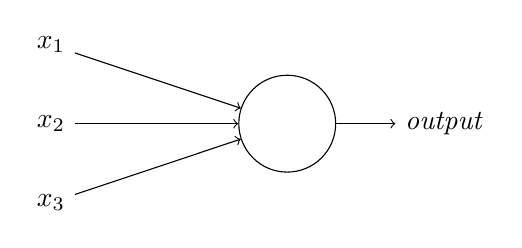
\begin{tikzpicture}[scale=1, transform shape]
\node (a)[circle, draw, minimum width=35pt] at (3, 0) {};
\node (x1)[] at (0, 1) {$x_1$};
\node (x2)[] at (0, 0) {$x_2$};
\node (x3)[] at (0, -1) {$x_3$};
\node (output)[] at (5, 0) {$\mathit{output}$};
\draw[->] (x1) -- (a) ;
\draw[->] (x2) -- (a) ;
\draw[->] (x3) -- (a) ;
\draw[->] (a) -- (output);
\end{tikzpicture}
\caption{An artificial neuron with input $x_1, x_2, x_3$ and one output.}
\label{fig:AN}
\end{figure}

To compute the output we assign to each input a weight, $w_1, \dots, w_n$. The weights represent the importance of the respective inputs to the output. The neuron's output, 0 or 1, is determined by whether the weighted sum $\sum^n_{i=1} w_i x_i$ is less than or greater than  threshold value $t$. Just like the weights, the threshold is a real number which is a parameter of the neuron. To put it in more precise algebraic terms:
\begin{equation}
\mathit{output} = g = \left\{\begin{matrix}
 0 & \text{if } \sum\limits_{i=1}^n w_i x_i < t\\
 1 & \text{if } \sum\limits_{i=1}^n w_i x_i \geq t
\end{matrix}\right.
\label{eq:AF_perceptron}
\end{equation}
This function is also called an \textit{activation function}, in further reading denoted with a $g$.

And that is all we need to create an artificial neuron. As we see in section \ref{sec:neuron_revisted}, the artificial neuron described here is a specific type of artificial neurons called a perceptron. When we understand the perceptron and networks of perceptrons it is easier to understand how other types of neurons work and why they exist.

We can now make an artificial neuron that can act as a logic gate (see figure \ref{fig:neuron_and_gate}, \ref{fig:neuron_or_gate} and \ref{fig:neuron_invert_gate}). By assigning the weights and the threshold we decide on the behaviour.

\begin{figure}[h!]
\centering
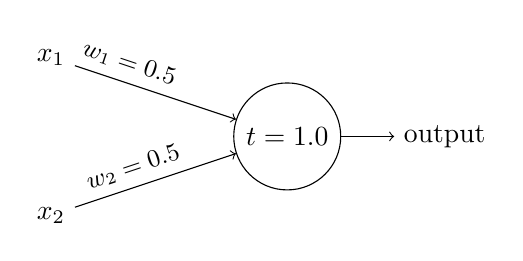
\begin{tikzpicture}[scale=1, transform shape]
\node (a)[circle, draw] at (3, 0) {$t = 1.0$};
\node (x1)[] at (0, 1) {$x_1$};
\node (x2)[] at (0, -1) {$x_2$};
\node (output)[] at (5, 0) {output};
\draw[->] (x1) -- (a) node[pos=0.3,sloped,above] {\small $w_1 = 0.5$};
\draw[->] (x2) -- (a) node[pos=0.4,sloped,above] {\small $w_2 = 0.5$};
\draw[->] (a) -- (output);
\end{tikzpicture}
%\caption{An perceptron given appropriate weights and threshold to act as an AND-gate.}
\caption{Appropriate weights and threshold to act as an AND-gate.}
\label{fig:neuron_and_gate}
\end{figure}
\begin{figure}[h!]
\centering
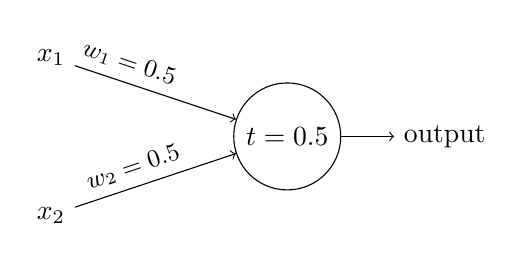
\begin{tikzpicture}[scale=1, transform shape]
\node (a)[circle, draw] at (3, 0) {$t = 0.5$};
\node (x1)[] at (0, 1) {$x_1$};
\node (x2)[] at (0, -1) {$x_2$};
\node (output)[] at (5, 0) {output};
\draw[->] (x1) -- (a) node[pos=0.3,sloped,above] {\small $w_1 = 0.5$};
\draw[->] (x2) -- (a) node[pos=0.4,sloped,above] {\small $w_2 = 0.5$};
\draw[->] (a) -- (output);
\end{tikzpicture}
% \caption{A perceptron given appropriate weights and threshold to act as an OR-gate}
\caption{Appropriate weights and threshold to act as an OR-gate.}
\label{fig:neuron_or_gate}
\end{figure}
\begin{figure}[h!]
\centering
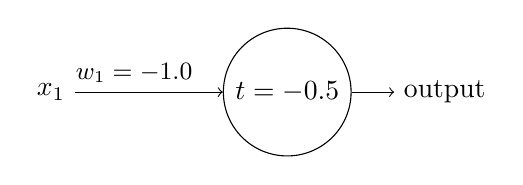
\begin{tikzpicture}[scale=1, transform shape]
\node (a)[circle, draw] at (3, 0) {$t = -0.5$};
\node (x1)[] at (0, 0) {$x_1$};
\node (output)[] at (5, 0) {output};
\draw[->] (x1) -- (a) node[pos=0.4,sloped,above] {\small $w_1 = -1.0$};
\draw[->] (a) -- (output);
\end{tikzpicture}
% \caption{A perceptron given appropriate weights and threshold to act as an INVERT-gate}
\caption{Appropriate weights and threshold to act as an INVERT-gate.}
\label{fig:neuron_invert_gate}
\end{figure}

\noindent
But we are not limited to logic gates. For example, we could make an artificial neuron that decides if we should go to a party. This decision can, of course, be made by weighing the following three factors:
\begin{itemize}
    \item Are your friends going?
    \item Are there cats at the party?
    \item Is the party free?
\end{itemize}
We can represent these three factors by corresponding binary variables $x_1$, $x_2$, and $x_3$. For instance, we'd have $x_1 = 1$ if your friends are going, and $x_1 = 0$ if your friends are not going. Similarly, $x_2=1$ if there are cats at the party, and $x_2=0$ if not. And similarly again for $x_3$ and whether there are entree costs to the party.

Suppose, that your friends make every party the best party possible, so much so that it doesn't matter if you have to pay or that there are no cats; you just have to be there. But if your friends are not there, the party needs to be free and have cats for you to be going. For this decision process we could use an artificial neuron. One way to do this is to choose a weight $w_1=0.6$ for the friends, a $w_2=0.3$ and $w_3=0.2$ for the other conditions and set the threshold $t$ to $0.4$. A larger value for the weight means that the factor matters more in the decision process. This unit can be seen in figure \ref{fig:party_unit}. By varying the weights and the threshold, we can get different models of decision-making. For instance, someone who thinks that cats are better than people (who doesn't?) might have a higher weight for $w_2$ and a lower weight for $w_1$.

\begin{figure}[h!]
\centering
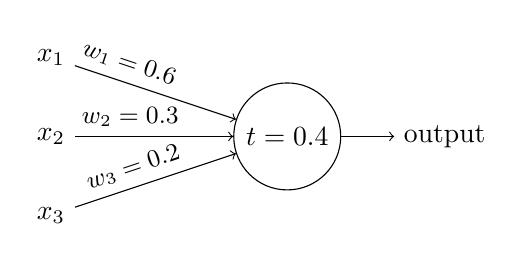
\begin{tikzpicture}[scale=1, transform shape]
\node (a)[circle, draw] at (3, 0) {$t = 0.4$};
\node (x1)[] at (0, 1) {$x_1$};
\node (x2)[] at (0, 0) {$x_2$};
\node (x3)[] at (0, -1) {$x_3$};
\node (output)[] at (5, 0) {output};
\draw[->] (x1) -- (a) node[pos=0.3,sloped,above] {\small $w_1 = 0.6$};
\draw[->] (x2) -- (a) node[pos=0.35,sloped,above] {\small $w_2 = 0.3$};
\draw[->] (x3) -- (a) node[pos=0.4,sloped,above] {\small $w_3 = 0.2$};
\draw[->] (a) -- (output);
\end{tikzpicture}
\caption{A possible perceptron to decide if we should go to a party.}
\label{fig:party_unit}
\end{figure}

\subsection{The limits of perceptrons}
We saw in the figures \ref{fig:neuron_and_gate}, \ref{fig:neuron_or_gate} and \ref{fig:neuron_invert_gate} that perceptrons can represent the simple Boolean functions AND, OR and NOT, but what are the limits to the Boolean functions that can be represented with an artificial neuron? When we look at the activation function in equation \ref{eq:AF_perceptron} we see that it is a linear function. If we would represent our decision making in a two-dimensional plot based on the values of two inputs, then we can only draw one straight line to separate the two decisions. This is shown in figure \ref{fig:linairseperabilty_AND} for an AND-gate. The white and black dots are linear separable. The line between the white and black dots represents the threshold. An artificial neuron can represent an AND-gate. A XOR-gate cannot be represented by an artificial neuron, as there is no single straight line that separates the white and the black dots (see figure \ref{fig:linairseperabilty_EXNOR}).

\begin{figure}
\centering
\begin{tikzpicture}[scale=1, transform shape]

\pgfdeclarelayer{bg}    % declare background layer
\pgfsetlayers{bg,main}  % set the order of the layers (main is the standard layer)

\node (a)[circle, draw, fill=white!30] at (0, 0) {};
\node (a)[circle, draw, fill=white!30] at (2, 0) {};
\node (a)[circle, draw, fill=white!30] at (0, 2) {};
\node (a)[circle, draw, fill=black] at (2, 2) {};

\begin{pgfonlayer}{bg}
\draw[->] (0,-0.5) -- (0,3.5);
\draw[->] (-0.5,0) -- (3.5,0) ;
\draw[-,dashed] (3.5,-0.5) -- (-0.5,3.5) ;
\end{pgfonlayer}
\end{tikzpicture}
\caption{A two-dimensional plot of the decision making for an AND-gate. }
\label{fig:linairseperabilty_AND}
\end{figure}

\begin{figure}
\centering
\begin{tikzpicture}[scale=1, transform shape]

\pgfdeclarelayer{bg}    % declare background layer
\pgfsetlayers{bg,main}  % set the order of the layers (main is the standard layer)

\node (a)[circle, draw, fill=white!30] at (0, 0) {};
\node (a)[circle, draw, fill=black] at (2, 0) {};
\node (a)[circle, draw, fill=black] at (0, 2) {};
\node (a)[circle, draw, fill=white!30] at (2, 2) {};

\begin{pgfonlayer}{bg}
\draw[->] (0,-0.5) -- (0,3.5);
\draw[->] (-0.5,0) -- (3.5,0) ;
%\draw[-] (3.5,-0.5) -- (-0.5,3.5) ;
\end{pgfonlayer}
\end{tikzpicture}
% \caption{A two-dimensional plot of the decision making for a XOR-gate. The white and black dots are not linear separable. An artificial neuron cannot represent an XOR-gate.}
\caption{Plot of decision making for a XOR-gate. The white and black dots are not linear separable.}
\label{fig:linairseperabilty_EXNOR}
\end{figure}

\section{A simple artificial neural network}
A perceptron has it limits in decision making and is in no way close to a complete model for (human) decision making, but, just like logic-gates (see figure \ref{fig:logic_adder}), we can combine them to make more subtle decisions. To get ourselves familiar with the terms used in neural networks we look in this section at the small network depicted in figure \ref{fig:small_perc_network}.

\begin{figure}
\centering
\includegraphics[scale=0.6]{adder}
\caption{An adder built out of NAND-gates.}
\label{fig:logic_adder}
\end{figure}

\begin{figure}
\centering
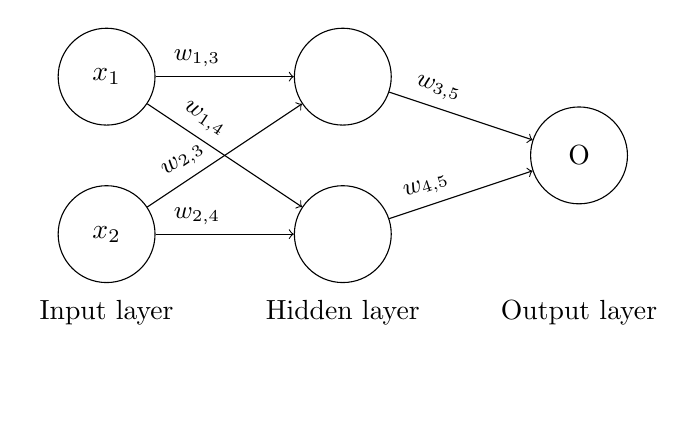
\begin{tikzpicture}[scale=1, transform shape]
\node (x1)[circle, draw, minimum width=35pt] at (0, 1) {$x_1$};
\node (x2)[circle, draw, minimum width=35pt] at (0, -1) {$x_2$};
\node (IL)[circle] at (0, -2) {Input layer};

\node (a)[circle, draw, minimum width=35pt] at (3, 1) {};
\node (b)[circle, draw, minimum width=35pt] at (3, -1) {};
\node (HL)[circle] at (3, -2) {Hidden layer};

\node (c)[circle, draw, minimum width=35pt] at (6, 0) {O};
\node (OL)[circle] at (6, -2) {Output layer};

\draw[->] (x1) -- (a) node[pos=0.3,sloped,above] {\small $w_{1,3}$};
\draw[->] (x1) -- (b) node[pos=0.3,sloped,above] {\small $w_{1,4}$};
\draw[->] (x2) -- (a) node[pos=0.3,sloped,above] {\small $w_{2,3}$};
\draw[->] (x2) -- (b) node[pos=0.3,sloped,above] {\small $w_{2,4}$};

\draw[->] (a) -- (c) node[pos=0.3,sloped,above] {\small $w_{3,5}$};
\draw[->] (b) -- (c) node[pos=0.3,sloped,above] {\small $w_{4,5}$};
\end{tikzpicture}
\caption{A small neural network. Weight $w_{i,j}$ is the weight of the link between unit $i$ and unit $j$.}
\label{fig:small_perc_network}
\end{figure}

\subsection{Units and layers}
Artificial neurons in networks are often called \textit{units}. In a network we can distinguish different type of units. The first layer of units with the input ($x_1$ and $x_2$ in figure \ref{fig:small_perc_network}) are called input units. These units do not get input from other units. Instead their activation depends on external variables (e.g. the grayscale of a pixel). The last layer of units in a network is called the output layer. The activation of the output units in this layer correspondents to the possible answers that we want to get out of the network (e.g., it is a cat). The layers between the input layer and the output layer are called hidden layers. A network without hidden layers is called a single-layer neural network (we do not count the input layer). Neural networks with one or more hidden layers are called multi-layer neural networks.

Layers are connected with each other by links, the connections between two units. As we already discussed, every input has a weight corresponding to it. We could rephrase that to say that every link has a corresponding weight. Where weight $w_{i,j}$ is the weight of the link between unit $i$ and unit $j$.

Note that, although a unit can have multiple outputs arrows, in reality a unit has only one output. Multiple arrows only depict that the output is transferred to multiple units.

\subsection{Feed-forward network}
The network seen in figure \ref{fig:small_perc_network} is a \textit{feed-forward network}. In a feed-forward network the links are unidirectional, and there are no cycles. Technically speaking, a feed-forward network is a directed acyclic graph (DAG). In more layman's terms, in a feed-forward network the activation of the units can only go to the next layer and not back to a previous layer. The significance of the lack of cycles is that computation can proceed uniformly from input units to output units. The activation from the previous time step (the last time the activation of the whole network was calculated) plays no part in the computation, because it is not fed back to an earlier unit. Hence, a feed-forward network simply computes a function of the input values that depends on the weight settings, it has no internal state other than the weights themselves. For instance, the function for the output of the network in figure \ref{fig:small_perc_network} would be:
\begin{equation}
\begin{split}
O & = g(w_{3,5}a_3 + w_{4,5}a_4)\\
       & = g(w_{3,5}g(w_{1,3}a_1 + w_{2,3}a_2) + w_{4,5}g(w_{1,4}a_1 + w_{2,4}a_2))
\end{split}
\end{equation}
where $g$ is the activation function (see section \ref{sec:ArtificialNeuron}), $w_{i,j}$ is the weight of the link between unit $i$ to unit $j$ and $a_i$ is the activation of unit $i$.

A more specific type of a feed-forward network is the \textit{layered feed-forward network}. In a layered feed-forward network each unit is linked only to units in the next layer. There are no links between units in the same layer, no links backward to a previous layer, and no links that skip a layer. The network in figure \ref{fig:small_perc_network} is also a layered feed-forward network.

Neural networks that have cycles and/or bidirectional links are called recurrent networks. Note that our brain is a recurrent network as we otherwise had no short-term memory. In this course, we focus on feed-forward networks because they are relatively well-understood.

\section{Artificial neuron revisited}
\label{sec:neuron_revisted}
The artificial neuron we described before is called a perceptron. There is another type of artificial neuron called a \textit{sigmoid neuron}. In this section we describe the sigmoid neuron, but before we look at the sigmoid neuron let us simplify how we describe perceptrons.

\subsection{Introducing Bias}%\todo{andere titel?}
In section \ref{sec:ArtificialNeuron} we described the working of a perceptron in equation \ref{eq:AF_perceptron} using inputs $x_1 \dots x_n$, corresponding weights $w_1 \dots w_n$ and threshold $t$. The condition $\sum_{i=1}^n w_i x_i > t$ is cumbersome, and we can make two notational changes to simplify it. The first change is to write it as a dot product, $\vec{w} \cdot \vec{x} = \sum_{i=1}^n w_i x_i$, where $\vec{w}$ and $\vec{x}$ are \textit{vectors} whose components are the weights and inputs, respectively. % \footnote{The $\equiv$ means that what is on the left side is equivalent to what is on the right side. In other words, $\vec{w} \cdot \vec{x}$ is the same as $\sum_{i=1}^n w_i x_i$.}

The second change is to move the threshold to the other side of the inequality, and to replace it by what's known as the perceptron's bias: $b = -threshold$. Using the bias instead of the threshold, the perceptron activation function, $g$, can be rewritten:

\begin{equation}
\mathit{output} = g = \left\{\begin{matrix}
 0 & \text{if } \vec{w} \cdot \vec{x} + b < 0\\
 1 & \text{if } \vec{w} \cdot \vec{x} + b \geq 0
\end{matrix} \right.
\label{eq:AF_perceptron_withbias}
\end{equation}

You can think of the bias as a measure of how easy it is to get the perceptron to output a 1. Or to put it in more biological terms, the bias is a measure of how easy it is to get the perceptron to fire. For a perceptron with a really big bias, it's extremely easy for the perceptron to output a 1. But if the bias is very negative, then it's difficult for the perceptron to output a 1.

We can simplify equation \ref{eq:AF_perceptron_withbias} and our calculations a bit more by making the bias a weight of the special input $x_0$ which will always be 1. This will give us the perceptron activation function, $g$,:

\begin{equation}
\mathit{output} = g = \left\{\begin{matrix}
 0 & \text{if } \vec{w} \cdot \vec{x} < 0\\
 1 & \text{if } \vec{w} \cdot \vec{x} \geq 0
\end{matrix}\right.
\label{eq:AF_perceptron_withbiasasweight}
\end{equation}
where $\vec{w}$ is the vector whose components are the weights $w_0 \dots w_n$, $\vec{x}$ is the vector whose components are the inputs $x_0 \dots x_n$, $w_0$ is called the bias weight, with $x_0 = 1$.

This change from threshold to bias simplifies the calculations needed in neural networks, as now only vector multiplications are required. Later, in Section \ref{ch:opencl}, this means that we can more easily offload the neural network calculations to the GPU for training.


\subsection{Sigmoid neuron}
To understand why we have sigmoid neurons and why they are what they are we have to look at what we expect from a learning algorithm for neural networks. Suppose we have a network of perceptrons that we like to learn to solve some problem. For example, the inputs to the network might be the raw pixel data from a scanned, handwritten image of a digit. We would like the network to learn weights such that the output from the network correctly classifies the digit. To see how learning might work, suppose we make a small change in some weight in the network. What we would like is for this small change in weight to cause only a small corresponding change in the output from the network. This property will make learning easier. In figure \ref{fig:small_perc_network_smallChangeInWeights} is schematically depicted what we want.

\begin{figure}
\centering
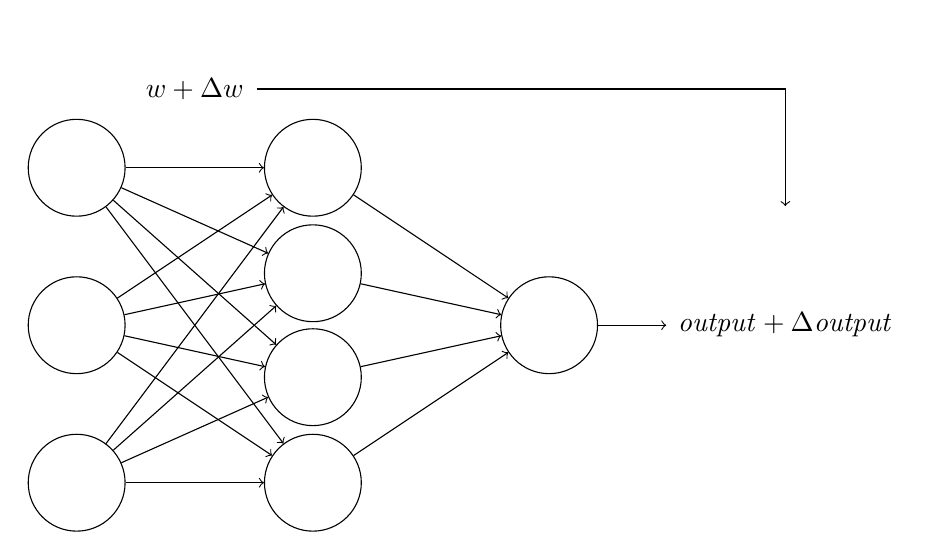
\begin{tikzpicture}[scale=1, transform shape]

\node (x1)[circle, draw, minimum width=35pt] at (0, 2) {};
\node (x2)[circle, draw, minimum width=35pt] at (0, 0) {};
\node (x3)[circle, draw, minimum width=35pt] at (0, -2) {};

\node (w)[circle] at (1.5, 3) {$w + \Delta w$};

\node (a)[circle, draw, minimum width=35pt] at (3, 2) {};
\node (b)[circle, draw, minimum width=35pt] at (3, 0.66) {};
\node (c)[circle, draw, minimum width=35pt] at (3, -0.66) {};
\node (d)[circle, draw, minimum width=35pt] at (3, -2) {};

\node (e)[circle, draw, minimum width=35pt] at (6, 0) {};

\node (output)[circle] at (9, 0) {$\mathit{output} + \Delta \mathit{output}$};

\draw[->] (x1) -- (a) node[pos=0.3,sloped,above] {};
\draw[->] (x1) -- (b) node[pos=0.3,sloped,above] {};
\draw[->] (x1) -- (c) node[pos=0.3,sloped,above] {};
\draw[->] (x1) -- (d) node[pos=0.3,sloped,above] {};
\draw[->] (x2) -- (a) node[pos=0.3,sloped,above] {};
\draw[->] (x2) -- (b) node[pos=0.3,sloped,above] {};
\draw[->] (x2) -- (c) node[pos=0.3,sloped,above] {};
\draw[->] (x2) -- (d) node[pos=0.3,sloped,above] {};
\draw[->] (x3) -- (a) node[pos=0.3,sloped,above] {};
\draw[->] (x3) -- (b) node[pos=0.3,sloped,above] {};
\draw[->] (x3) -- (c) node[pos=0.3,sloped,above] {};
\draw[->] (x3) -- (d) node[pos=0.3,sloped,above] {};


\draw[->] (a) -- (e) node[pos=0.3,sloped,above] {};
\draw[->] (b) -- (e) node[pos=0.3,sloped,above] {};
\draw[->] (c) -- (e) node[pos=0.3,sloped,above] {};
\draw[->] (d) -- (e) node[pos=0.3,sloped,above] {};

\draw[->] (e) -- (output) node[pos=0.3,sloped,above] {};

\draw[->] (w) -| (output) {};

\end{tikzpicture}
\caption{A small neural network. To be able to have an algorithm that can train a neural network, we want a small change in the weights, $w$, results in a small change in the output.}
\label{fig:small_perc_network_smallChangeInWeights}
\end{figure}

If it were true that a small change in a weight causes only a small change in output, then we could use this fact to modify the weights and biases to get our network to behave more in the manner we want. For example, suppose the network was mistakenly classifying an image as an ``8'' when it should be a ``9''. We could figure out how to make a small change in the weights and biases so the network gets a little closer to classifying the image as a ``9''. And then we can repeat this, changing the weights over and over to produce better and better output. The network would be learning.

The problem is that this is not what happens when our network contains perceptrons. In fact, a small change in the weights or bias of any single perceptron in the network can sometimes cause the output of that perceptron to completely flip, say from 0
to 1. That flip may then cause the behaviour of the rest of the network to completely change in some very complicated way. So while a ``9'' might now be classified correctly, the behaviour of the network on all the other images is likely to have completely changed in some hard-to-control way. That makes it difficult to see how to gradually modify the weights and biases so that the network gets closer to the desired behaviour.

We can overcome this problem by introducing a new type of artificial neurons called sigmoid neurons. Sigmoid neurons are similar to perceptrons, but modified such that small changes in their weights and bias cause only a small change in their output. That is the crucial fact which allows a network of sigmoid neurons to learn.

Just like a perceptron, the sigmoid neuron has an input vector $\vec{x}$ and a vector, $\vec{w}$, with weights for each connection. The big difference is that the possible inputs and output of a sigmoid neuron are not only 0's and 1's. The inputs and the output can take any value between 0 and 1. For instance, the value 0.563 is a valid input. To make this also possible for the output the sigmoid neuron uses a different activation function, $g$,:

\begin{equation}
\mathit{output} = g = \sigma(\vec{w} \cdot \vec{x})
\label{eq:AF_sigmoid_withbiasasweight}
\end{equation}
where $\sigma$ is called the \textit{sigmoid function}\footnote{Incidentally, $\sigma$ is sometimes called the logistic function, and this new class of neurons called logistic neurons. It is useful to remember this terminology, since these terms are used by many people working with neural networks. However, we stick with the sigmoid terminology.}, and is defined by:

\begin{equation}
\sigma(z) = \frac{1}{1+e^{-z}}
\label{eq:sigma_function}
\end{equation}

Figure \ref{fig:sigmoid_plot} (left) shows a plot of the sigma function. We can see that it is a smoothed version of the activation function of the perceptron (also called \textit{step-function}, see Figure \ref{fig:sigmoid_plot} (right)). This means that we can represent the same functions as with the perceptrons (such as AND-gates, etc.). Furthermore, we have the desired feature for a learning algorithm: a small change in weights results in a small change in output.

\begin{figure}
\centering
\includegraphics[width=0.45\textwidth]{sigmoid_function_plot}
\hfill
\includegraphics[width=0.45\textwidth]{perceptron_function_plot}
\caption{A plot of the sigmoid function (left) and step-function (right).}
\label{fig:sigmoid_plot}
\end{figure}

% \begin{figure}
% \centering
% \includegraphics[scale=0.5]{perceptron_function_plot}
% \caption{A plot of the activation function of a perceptron.}
% \label{fig:perceptron_plot}
% \end{figure}

\section{Neural networks and learning}
In the previous sections we collected all the parts to create a neural network. To make a learning neural network we only miss two things: examples to learn the task and a learning algorithm. Examples to learn from are called the \textit{training set}. This consists of a set of inputs and the desired outcomes. For instance, in the case of number recognition, a set with images of numbers (input) each with a label of which number it is (desired output). This section explains how a neural network can learn when it has a training set.

\begin{figure}[h!]
\centering
\includegraphics[width=0.8\textwidth, trim={1mm 1mm 1mm 1mm}, clip]{mnistExamples.png}
\caption{A selection of the MNIST training set of handwritten digits.}\label{fig:mnist}
\end{figure}

\subsection{Cost function}
\label{sec:cost_function}
To learn humans need feedback. This is also true for neural networks. The function that tells the neural network how good it is doing is called the \textit{cost function}. There are multiple types of functions than can be used as a cost function. Here, we use the mean squared error (MSE), also known as the quadratic cost function:

\begin{equation}
MSE = \frac{1}{n} \sum_{i=0}^n \left | \vec{y}_i - \vec{a}(\vec{x}_i) \right |^2
\label{eq:MSE}
\end{equation}

The formula for this cost function $C(\vec{w})$ calculates the error (cost $C$) given a vector of weights ($\vec{w}$):\footnote{The math for this cost function might seem complicated, but with a closer look we see it is literally the mean squared error. $\left | \vec{y_i} - \vec{a}(x_i) \right |$ is the difference (or distance) between the output that is given and the output that we want when given input $\vec{x}_i$. In other words $\left | \vec{y}_i - \vec{a}(x_i) \right | $ tells us how wrong the neural network is (i.e. how big the error is) when given input $\vec{x}_i$. As this value can be negative or positive and we are only interested in how wrong the neural network is, we square this value to make all values positive. This is the squared error part of the mean squared error. To get to MSE, we need to calculated the mean. This is done by summing ($\sum$) the squared error over all training inputs and dividing it by the number of training inputs, $i=1,\ldots,n$, ($\frac{1}{2n}$). Actually we also divide by two (hence the 2 in $\frac{1}{2n}$). This has no effect on the functionality when minimising the function, but it makes the function derivative easier. As we use the derivative of this function this  saves us some clutter. In short the MSE is nothing more than the average squared distance between the output of the neural network and the desired output.}

%\note{It is not clear (nor explained) what the $w$ is in $C(w)$. Moreover, we take a range from $1\dots n$, but this is not shown in the RHS of the formula; shouldn't we include an index $i$? And finally, $y$ and $a(x)$ are vectors (values of all output neurons)? If so, for consistency with the rest, they should get a $\vec{ }$.}

\begin{equation}
C(\vec{w}) = \frac{1}{2} MSE = \frac{1}{2n} \sum_{i=0}^n \left | \vec{y}_i - \vec{a}(\vec{x}_i) \right |^2
\label{eq:MSE}
\end{equation}
where $n$ is the number of training inputs, $x$, $\vec{y}_i$ is the desired outcome of the network when $\vec{x}_i$ is the input and $\vec{a}(x_i)$ is the output of the neural network when $\vec{x}_i$ is the input. The notation $\left | \vec{v} \right |$ denotes the usual length function for a vector $\vec{v}$. \footnote{If we have a vector $\vec{v}$ with values $v_1$, $v_2$ and $v_3$, then $\left | v \right |$ is equals to $ \sqrt{{v_1}^2+{v_2}^2+{v_3}^2}$.}

Inspecting the form of the quadratic cost function, we see that $C(\vec{w})$ is non-negative, since every term in the sum is non-negative. Furthermore, the cost $C(\vec{w})$ becomes small, i.e., $C(\vec{w})\approx 0$, precisely when $\vec{y}_i$ is approximately equal to the output, $\vec{a}$, for all training inputs, $\vec{x}_i$. So our training algorithm has done a good job if it can find weights and biases so that $C(\vec{w})\approx0$. By contrast, it's not doing so well when $C(\vec{w})$ is large - that would mean that $\vec{y}_i$ is not close to the output $\vec{a}$ for a large number of inputs. So the aim of our training algorithm will be to minimise the cost $C(\vec{w})$ as a function of the weights and biases. In other words, we want to find a set of weights and biases which make the cost as small as possible\footnote{For some readers the questions might rise why we try to minimise the quadratic cost function, as we just as well could maximise the number of correct classified training samples. The problem with the number of correct classified training samples is that it is not a smooth function. Making a small change in the weights of the units will most of the time result in no change in the number of correct classified training samples. This makes it hard to find which change we should make to the weights of the network. The quadratic cost function is smooth and, therefore, does not have this problem.}.

\subsection{Gradient descent}\label{sec:gradient}
In section \ref{sec:cost_function}, we saw that the goal of a learning algorithm is to minimise the cost function $C(\vec{w})$. As $\vec{w}$ consists out of a lot of weights it takes too much time to calculated for each possible $\vec{w}$ the value of $C(\vec{w})$ to see where $C(\vec{w})$ has the lowest value. A solution for this problem is to use gradient descent. Gradient descent is an optimisation algorithm that approaches a (local) minimum of a function by taking steps in the direction of the negative of the gradient of the function at the current point.

For a first understanding of this algorithm, imagine a blind woman on a mountain that has as goal to go the valley (a minimum). The blind woman doesn't know where she is and can't look around to see which way she has to go. As a solution she feels around to find the slope of the mountain. Now she knows where the mountain goes down and she takes a step in that direction. By repeating this for each step, until she cannot go further down, she knows she ends in a (local) minimum.

Another way to visualise this technique can be seen in figure \ref{fig:valley_with_ball}. The plane is the cost function with weights $v_1$ and $v_2$. A ball is placed at a random place on the plane. The ball is moved a small step into the direction it would roll. This is repeated until we reach the minimum of the plane. When the minimum is reached we have the desired values for $v_1$ and $v_2$.

\begin{figure}
\centering
\includegraphics[scale=0.5]{valley_with_ball}
\caption{Gradient descent can be seen as taking small steps in the direction a ball would roll, until you reach a minimum.}
\label{fig:valley_with_ball}
\end{figure}

Back to our problem. We cannot calculate the minimum of the function, but we can start at a random position (random weights) and then use gradient descent to move down to a minimum. More formal, the algorithm starts with a random $\vec{w}$ and calculates which small change, $\Delta \vec{w}$, reduces $C(\vec{w})$. In other words, we want to find a $\Delta \vec{w}$, that has a negative $\Delta C(\vec{w})$. When $\Delta \vec{w}$ is applied to the weights $C(\vec{w})$ comes closer to a minimum. When we keep repeating this step until we cannot find a $\Delta \vec{w}$, such that $\Delta C(\vec{w})$ is negative, than we are at a (local) minimum and the network has learned its weights.

The $\Delta \vec{w}$ can be found by calculating the gradient on our current position, $\vec{w}$. The gradient can be found by using the derivatives\footnote{If you are not familiar (anymore) with what a derivative is we recommend watching the first 3 chapters of ``essence of calculus'' by 3Blue1Brown that can be found on youtube: \url{https://youtu.be/WUvTyaaNkzM}.} over each weight. The collection of the gradients is called the gradient vector, $\nabla C$:
\begin{equation}
\nabla C = \left (  \frac{\partial C}{\partial w_1}, \dots, \frac{\partial C}{\partial w_n} \right )^T
\end{equation}
where $\frac{\partial C}{\partial w_i}$ is the gradient over weight $w_i$ and note that $T$ here is the transpose operation, turning a row vector into an ordinary (column) vector.

Gradient descent tells us that if we move the weights in the negative direction of $\nabla C$, then we move in the direction of a (local) minimum. With this we can create an update rule that tells us that in each step our new weights, $\vec{w}'$, become:
\begin{equation}
\vec{w}'= \vec{w} - \Delta \vec{w} = \vec{w} - \eta \nabla C
\end{equation}
where $\eta$ is called the learning rate and denotes the size of the step we take in the direction of $-\nabla C$. When $\eta$ is too large we might overshoot a minimum, but a too small $\eta$ requires a lot of steps making the algorithm very slow.

Without vectors, which might make it easier to understand, the update rule for weight $w_i$ is:
\begin{equation}
w_i'= w_i - \Delta w_i = w_i - \eta \frac{\partial C}{\partial w_i}
\end{equation}

\subsection{Single-layer network}
From the last section we know that we can train our neural networks using gradient descent and that we can do that using the derivatives of the cost function. But what are these derivatives? Here we work towards the update rule for our weights for single layer networks. In the next section we generalise this rule to work for multi-layer networks.

First take a look again at the cost function (see equation \ref{eq:MSE}). It requires to look at all training examples for each step. This is a big calculation just for one step. To make our training algorithm faster (but a bit less accurate), we take a step after each training example. The cost function for just one training example is:
\begin{equation}
C = \frac{1}{2} \left | \vec{y} - \vec{a}(\vec{x}) \right |^2
\end{equation}

Now we can use gradient descent to reduce the squared error\footnote{Note that we no longer have to calculate the mean of the squared error, as we are only looking at a single example.} by calculating the partial derivative of $C$ with respect to each weight and updating the weight:
\begin{equation}
\begin{split}
w_i' & = w_i - \eta \frac{\partial C}{\partial w_i} \\
& = w_i - \eta \frac{\partial(\frac{1}{2} \left | \vec{y} - \vec{a}(\vec{x}) \right |^2)}{\partial w_i}
\end{split}
\end{equation}

In a single layer network (see figure \ref{fig:single_layer_neural_network}) each weight has a direct influence on one of the output nodes. The update rule can therefore be rewritten for the weight from input node $j$ to output node $k$:%\todo{Moet dit nog verder uitgewerkt worden?}

\begin{equation}
w_{j,k} = w_{j,k} - \Delta w_{j,k} = w_{j,k} + \eta a_{j} g'(in_k)(y_k - a_k)
\end{equation}
where $a_j$ is the activation of input node $j$, $g'$ is the derivative of the activation function \footnote{For the sigmoid neuron the derivative is given by $g' = g(1-g)$}, $in_k$ is the summed input of output node $k$, $y_k$ is the desired activation of output node $k$ and $a_k$ is the actual activation of output node $k$\footnote{Note the change of sign in the equation: the (partial) derivative $\eta \frac{\partial(\frac{1}{2} \left | \vec{y} - \vec{a}(\vec{x}) \right |^2)}{\partial w_i}$ is negative (as we are looking for the down slope), which means that the sign changes from a minus to a plus.}. This updating rule is called the \textit{delta rule}.

The learning algorithm starts by assigning random values to the weights. Then it keeps updating the weights using the delta rule. Note that the update of the weights happens simultaneously. So, first are all $\Delta w_{j,k}$ calculated and then are all weights updated using the $\Delta w_{j,k}$'s. When a minimum is reached the algorithm stops.

\begin{figure}
\centering
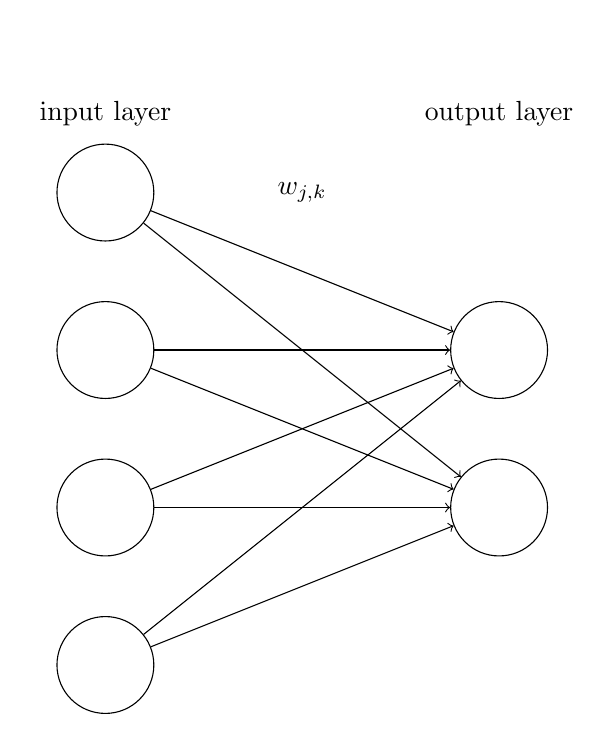
\begin{tikzpicture}[scale=1, transform shape]

\node (input)[circle] at (0, 3) {input layer};

\node (x1)[circle, draw, minimum width=35pt] at (0, 2) {};
\node (x2)[circle, draw, minimum width=35pt] at (0, 0) {};
\node (x3)[circle, draw, minimum width=35pt] at (0, -2) {};
\node (x4)[circle, draw, minimum width=35pt] at (0, -4) {};

\node (output)[circle] at (2.5, 2) {$w_{j,k}$};

\node (output)[circle] at (5, 3) {output layer};
\node (a)[circle, draw, minimum width=35pt] at (5, 0) {};
\node (b)[circle, draw, minimum width=35pt] at (5, -2) {};


\draw[->] (x1) -- (a) node[pos=0.3,sloped,above] {};
\draw[->] (x1) -- (b) node[pos=0.3,sloped,above] {};
\draw[->] (x2) -- (a) node[pos=0.3,sloped,above] {};
\draw[->] (x2) -- (b) node[pos=0.3,sloped,above] {};
\draw[->] (x3) -- (a) node[pos=0.3,sloped,above] {};
\draw[->] (x3) -- (b) node[pos=0.3,sloped,above] {};
\draw[->] (x4) -- (a) node[pos=0.3,sloped,above] {};
\draw[->] (x4) -- (b) node[pos=0.3,sloped,above] {};


\end{tikzpicture}
\caption{A single layer neural network}.
\label{fig:single_layer_neural_network}
\end{figure}

\subsection{Multi-layer network}
In multi-layer networks we have the problem that the weights to hidden layers do not directly influence the output. To  be able to also train these weights we take the idea that hidden node $j$ is ``responsible'' for some fraction of the error in the layer after it. To get to our update rule for the hidden layers we rewrite the delta rule to emphasise what we see as the error:

\begin{equation} \label{eq_output_error}
\Delta_k = g'(in_k)(y_k - a_k)
\end{equation}
\begin{equation}
w_{j,k} = w_{j,k}' + \eta a_j \Delta_k
\end{equation}
where $\Delta_k$ is the error of output node $k$.

If we would know $\Delta_j$, the fraction of error that hidden node $j$ is responsible of in all output nodes, then we can rewrite the update rule to get the update rule for the weights from node $i$ to hidden node $j$:
\begin{equation}
w_{i,j} = w_{i,j}' + \eta a_i \Delta_j
\end{equation}
where $a_i$ is the activation of node $i$. This looks quite similar as the rule for the weights to the output layer. We can calculate $\Delta_j$ with:

\begin{equation} \label{eq:hiddenlayerDeltaerror}
\Delta_j = g'(in_j) \sum_p w_{j,p}\, \Delta_p
\end{equation}
where $w_{j,p}$ is the weight from node $j$ to node $p$ and $\Delta_p$ is the error of node $p$. If node $p$ is an output node then $\Delta_p$ is calculated as $\Delta_k$ in equation \ref{eq_output_error} otherwise it is calculated the same way as $\Delta_j$. In the formula for $\Delta_j$ we see that node $j$ is held ``responsible'' for the error in the nodes it is connected to in the next layer dependent on its activation and its weights.

The algorithm is similar to that of the single-layer networks. The algorithm starts by assigning random values to the weights. Then for each example in the training set it calculates the activation for each node. As the activation of a node depends on the activation of the nodes of the previous layer, this is called forward propagation (the activation moves from the input layer to the output layer). Then the error deltas ($\Delta$) for each node are calculated. As these are dependent on the next layer the delta calculation moves from the output layer to the input layer. The error propagates back through the network. When the deltas are known the weights are updated. One loop over all training samples is called an \textit{epoch}. This is repeated for multiple epochs until some stopping criterion (such as a minimum in the cost function) is reached. This algorithm is called \textit{backpropagation} named after the back propagation of the errors.

\section{Exercises}
\begin{exercise}[NOR-Gate]~\label{ex:NOR-Gate}\\
Determine weights and a threshold for a perceptron that would act as a NOR-gate with three inputs.

%Anwser NOR: $ t = -1$, $w_1 = -2$, $w_2 = -2$ and $w_3 = -2$
\end{exercise}

\begin{exercise}[Neural ADDER]~\label{ex:ADDER}\\
Make an adder out of perceptrons. Draw the network and give the corresponding weights and biases.

%Anwser: \ref{fig:perceptron_adder} all NAND-perceptrons: $ t = -3$, $w_1 = -2$, $w_2 = -2$
\end{exercise}

% \begin{figure}[h!]
% \centering
% \begin{tikzpicture}[scale=0.8, transform shape]
% \node (x1)[circle, draw, minimum width=35pt] at (0, 1) {$x_1$};
% \node (x2)[circle, draw, minimum width=35pt] at (0, -1) {$x_2$};
%
% \node (a)[circle, draw, minimum width=35pt] at (3, 0) {};
%
% \node (b)[circle, draw, minimum width=35pt] at (6, 1) {};
% \node (c)[circle, draw, minimum width=35pt] at (6, -1) {};
% \node (d)[circle, draw, minimum width=35pt] at (6, -3) {};
%
% \node (e)[circle, draw, minimum width=35pt] at (9, 0) {};
%
% \node (sum)[] at (12, 0) {sum: $x_1 \bigoplus x_2$};
% \node (carry)[] at (12, -3) {carry bit: $x_{1} x_{2}$};
%
% \draw[->] (x1) -- (a);
% \draw[->] (x2) -- (a);
%
% \draw[->] (x1) -- (b) ;
% \draw[->] (x2) -- (c) ;
%
% \draw[->] (a) -- (b) ;
% \draw[->] (a) -- (c) ;
% \draw[->, double distance=2pt] (a) -- (d) ; %I don't really like this double line. Solutions? - Jorn
%
% \draw[->] (b) -- (e);
% \draw[->] (c) -- (e);
% \draw[->] (d) -- (carry);
%
% \draw[->] (e) -- (sum);
% \end{tikzpicture}
% \caption{An adder built from perceptrons}.
% \label{fig:perceptron_adder}
% \end{figure}

\begin{exercise}[Programming NNs]~\\
In this exercise you are going to build a (naive) implementation of a neural networks\footnote{In the next section we discuss a ``smarter'', more mathematical, implementation of neural networks.} and use it to classify a number of data sets.

\paragraph{A) Neuron}
Write a class to represent a neuron and its functions. Learning capabilities are not necessary yet. Use this class to implement the neuron of exercise \ref{ex:NOR-Gate} and the network of exercise \ref{ex:ADDER}.

\paragraph{B) Delta Rule}
Add to the neuron class an update function. This function uses the delta rule to updates its weights. The function has as input the desired activation of the node. Test your new function to train the neuron of exercise \ref{ex:NOR-Gate}.

\paragraph{C) Backpropagation}
Add backpropagation to your program. Create the XOR network from the sheets. Initialize the weights with random values. Train the network.

\paragraph{D) Iris dataset}
Create a neural network, using your own code, that is able to classify correctly a high percentage of flowers from the iris dataset\footnote{\url{http://archive.ics.uci.edu/ml/datasets/Iris}}. Make sure you use a train set and a test set.

\noindent
Report the shape of your network and its score on the test set.

\paragraph{E) Weather data [optional]}
Adjust your implementation to work on the weather data from the previous chapter. Can your NN perform as well as (or better than) your $k$-NN implementation?
\end{exercise}
